\section{Experimental Setup}
\label{experimental_setup}

In \Cref{fig:fish_CAD}, we show renderings of the three types of fishtail actuators we investigate in this work. We vary material parameters as well as geometry.

\begin{figure}
    \centering
    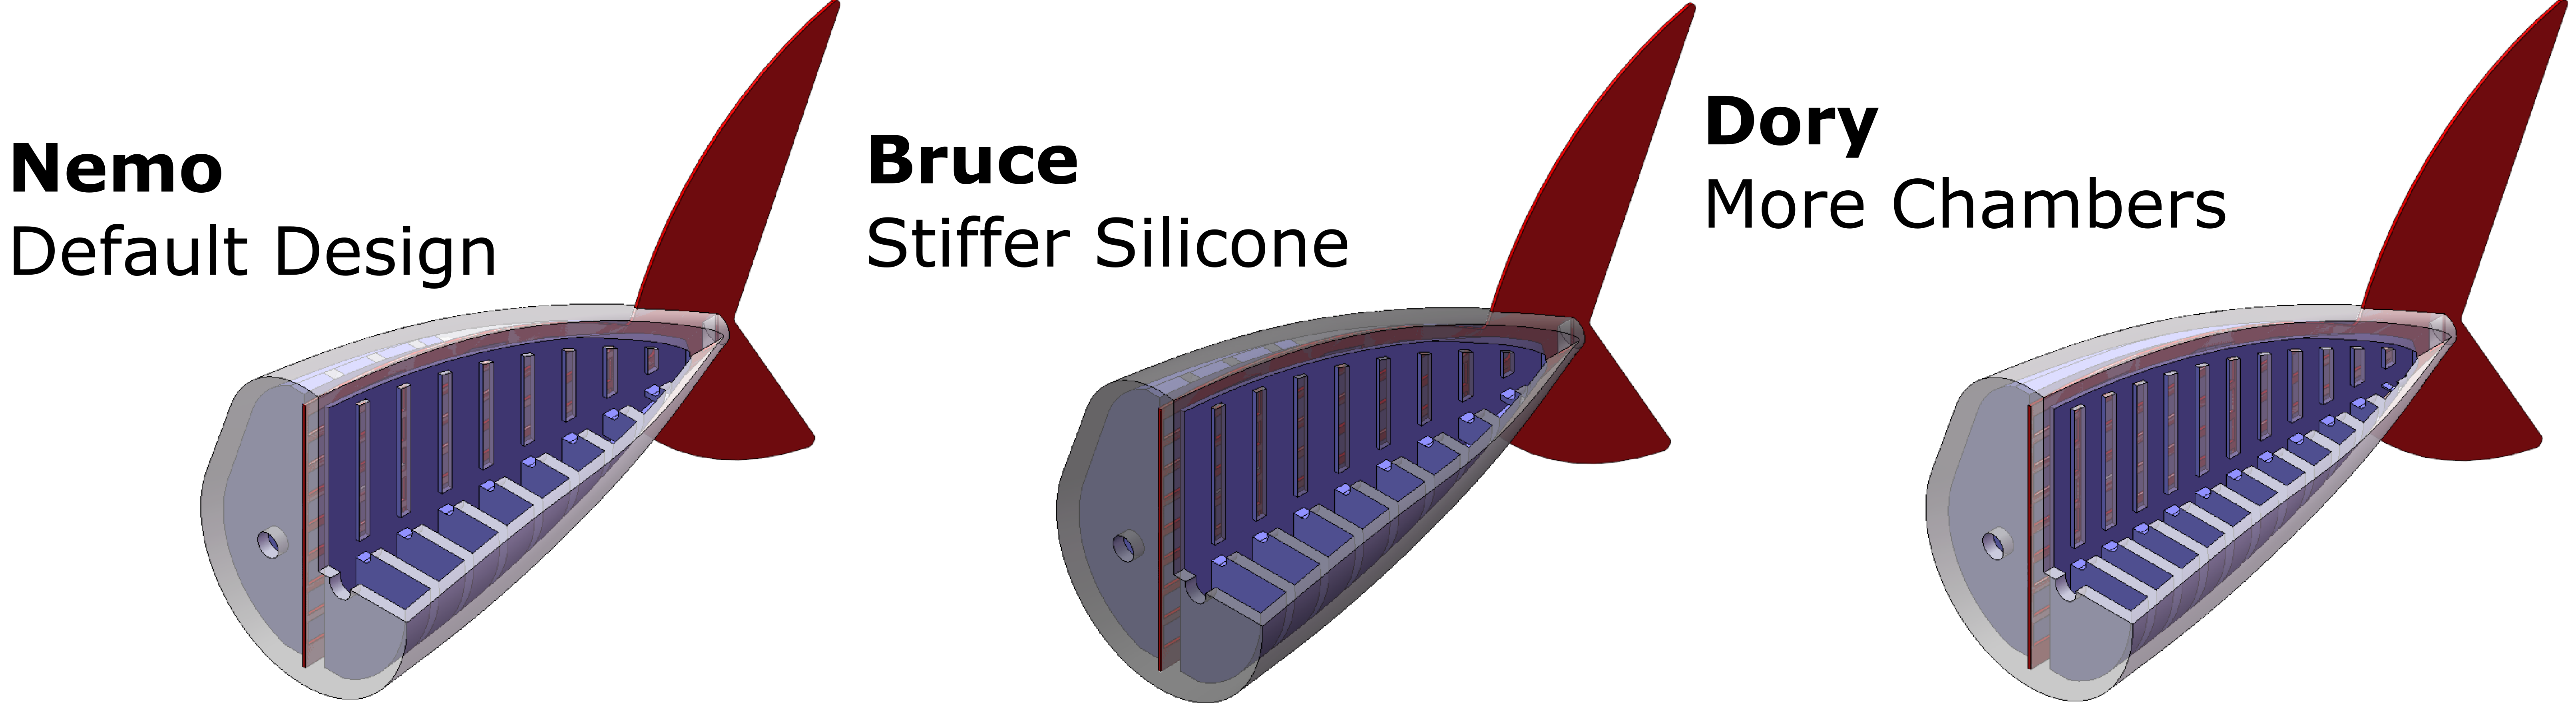
\includegraphics[width=\linewidth]{figures_appendix/fish_CAD_horiz.png}
    \caption{Three different actuator designs. \emph{Nemo} and \emph{Bruce} share the same geometry but \emph{Bruce} has a stiffer DS20 material for its body. \emph{Nemo} and \emph{Dory} share the same materials but \emph{Dory} has a greater number of air chambers.}
    \label{fig:fish_CAD}
\end{figure}

We collect tail deformation, thrust force, and air chamber pressure data of pneumatically actuated silicone fishtail both in air and in water. To this end, the fishtail is mounted in a water tank and the fish head is rigidly connected to a load cell (TAL2210, \SI{1}{kg} model) to measure the thrust force in the heading direction (\Cref{fig:experimental_setup}). The load cell data is obtained using an amplifier board and a microcontroller.\footnote{Amplifier: HX711, Microcontroller: Arduino Leonardo} Black markers are painted onto the fish’s back and tracked using Kanade-Lucas-Tomasi (KLT) feature tracking in a video captured from above using a GoPro Hero 6 camera~\cite{lucas1981iterative,tomasi1991tracking}. We found in practice that three markers are sufficient for capturing the deformation of the fishtail and can be used as input to our learning pipeline. From the video after correcting for parallax and distortion, we obtain in-plane displacements for each marker. An LED is used to synchronize the pressure and the force data with the recorded video. The fish is actuated with a Festo proportional valve manifold with controlled pressure\footnote{MBA-FB-VI, \SI{0}-\SI{2}{bar} range, 1\% accuracy}, which outputs desired and actual pressure data for both air chamber sides of the fishtail.

\begin{figure}[tb]
    \centering
    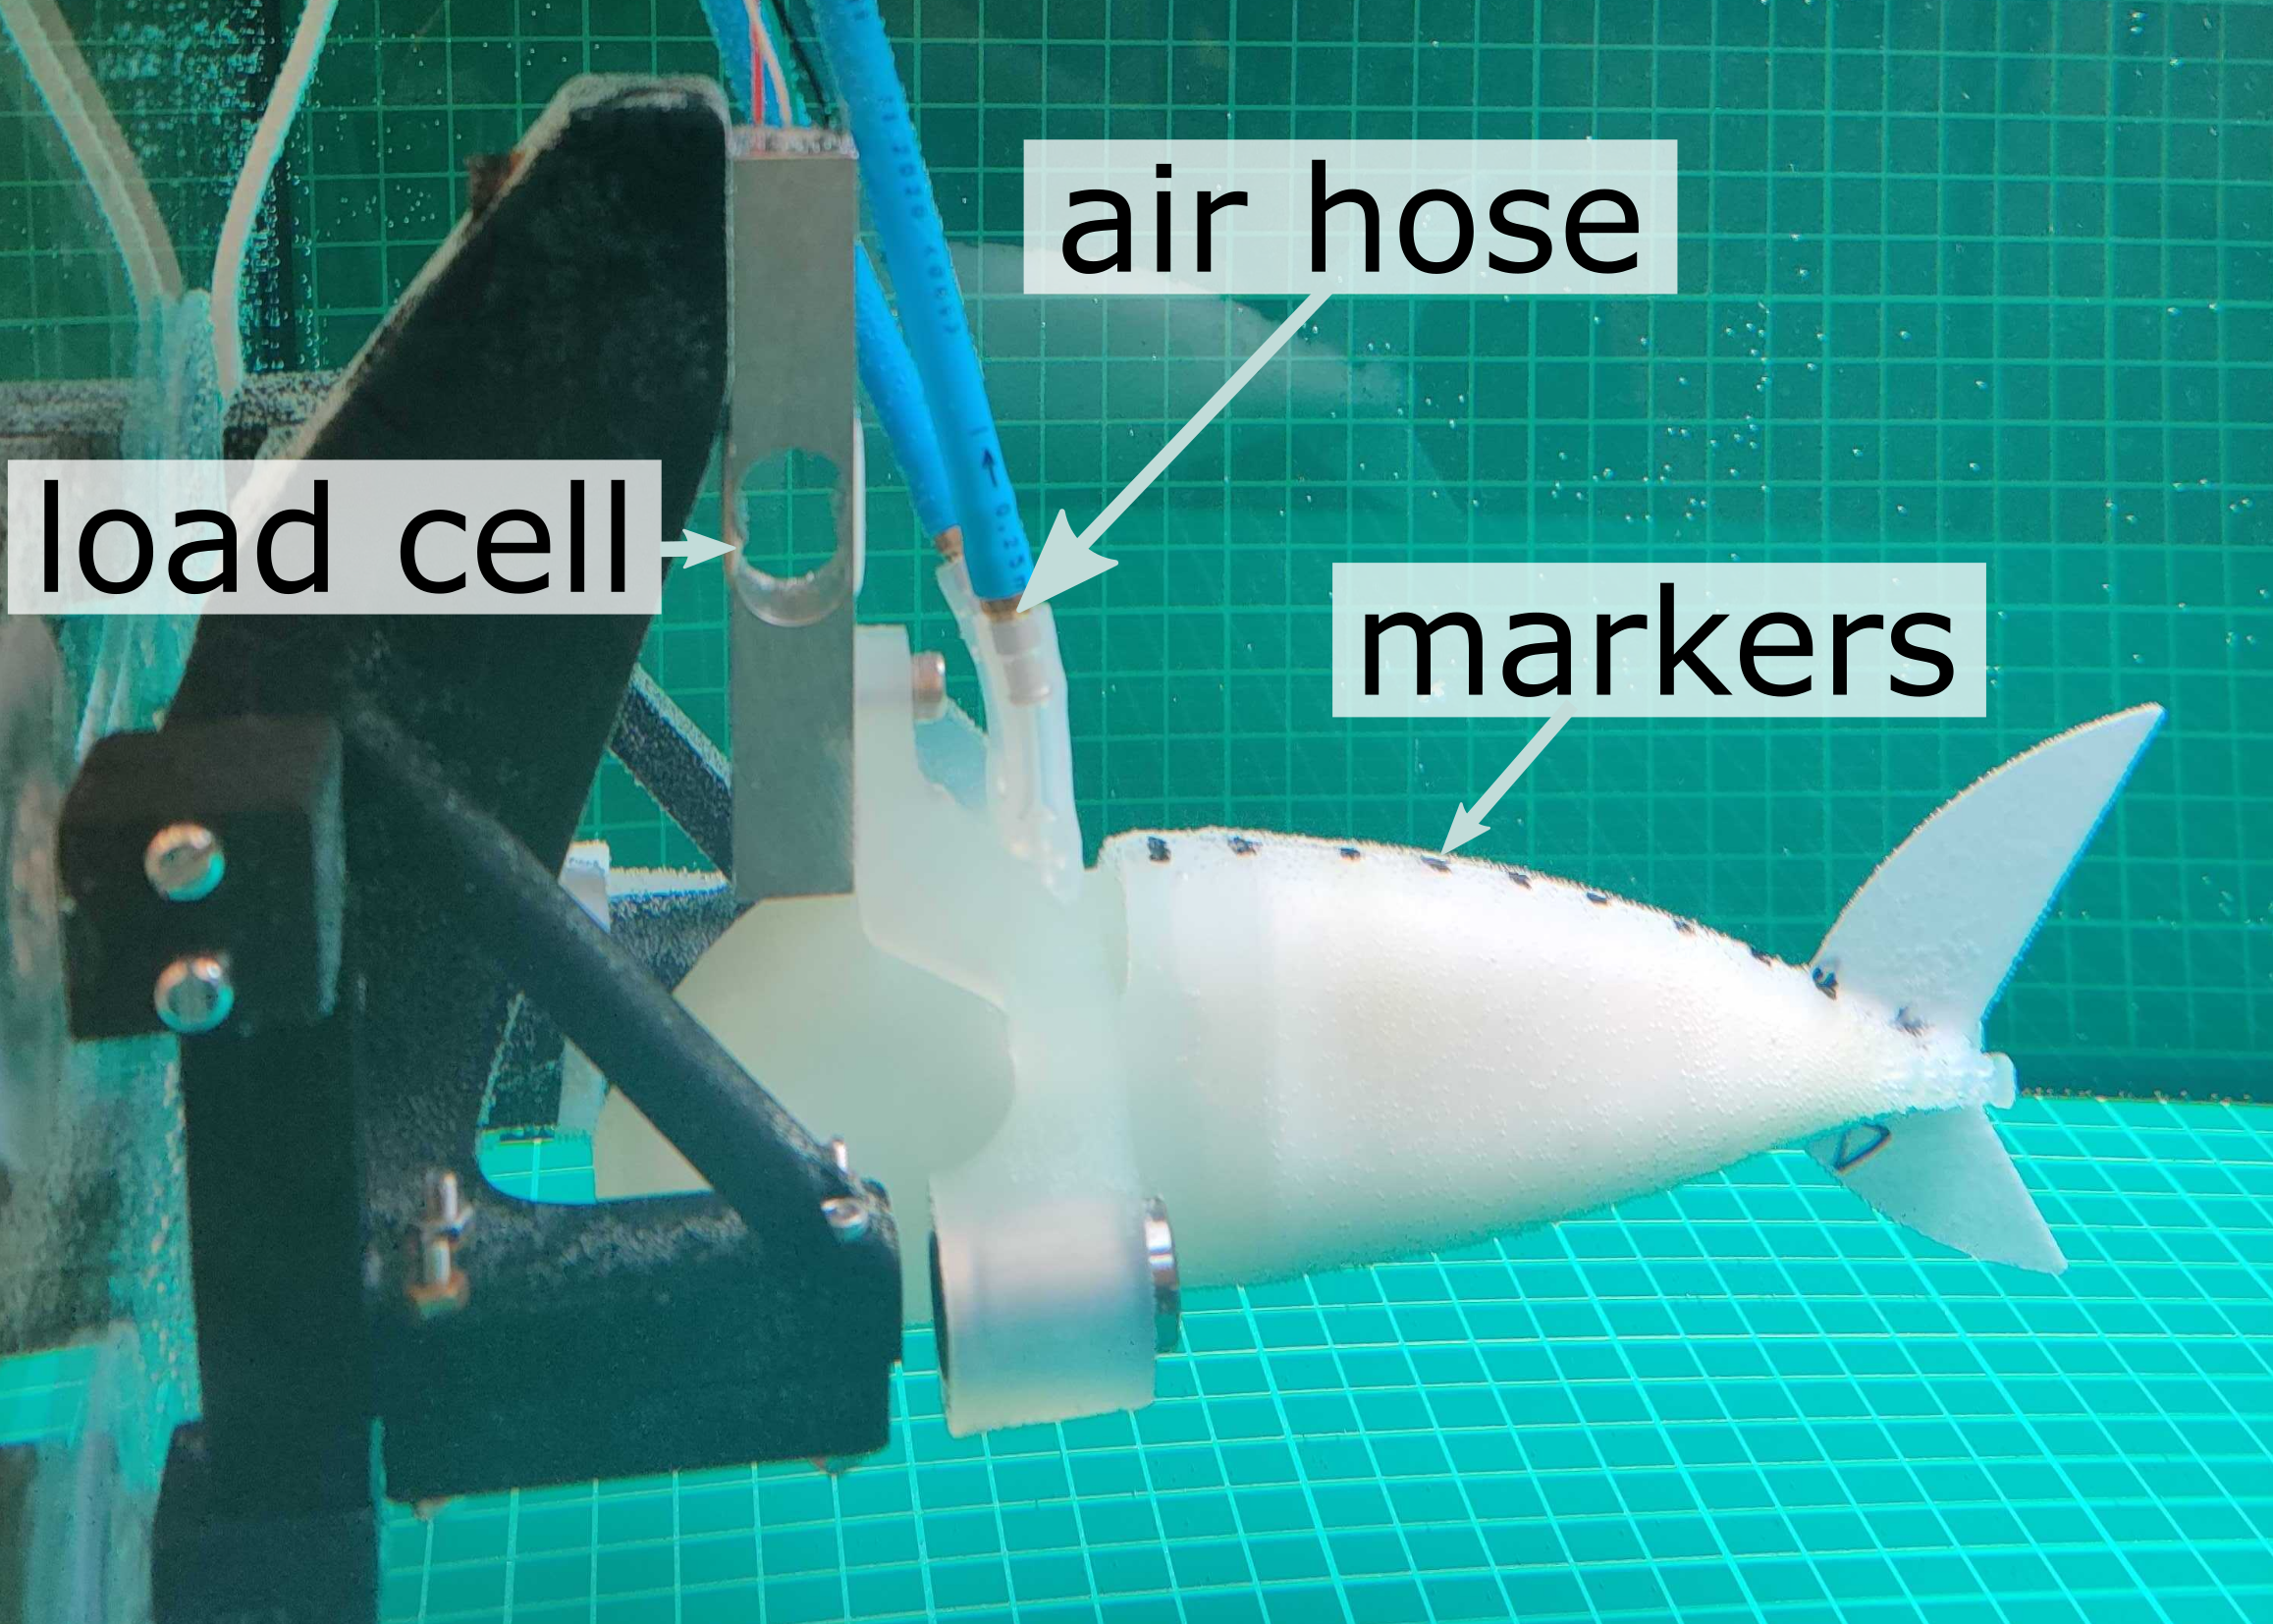
\includegraphics[width=0.65\columnwidth]{figures/experimental_setup_v2.png}
    \caption{Thrust experiment setup actuated with a Festo proportional valve manifold. A 3D-printed fixture (black) connects the load cell (grey) to a fish adapter (opaque). The fish adapter is mounted within a casted soft robotic fish tail made of silicone elastomer. The deformation of the tail is captured using a GoPro positioned above the tail. Markers on the back of the fish are tracked using Kanade-Lucas-Tomasi (KLT) feature tracking. The thrust generated by the fish is measured using a load cell.}
    \label{fig:experimental_setup}
\end{figure}
\begin{table}[t]
    \centering
    \caption{Material, Young's moduli, air chambers, and maximum applied pressure for each prototype. Reported material parameters are nominal values.}
    % \begin{tabular}{| p{1.5cm}| p{0.7cm} p{0.7cm} p{0.7cm}|} 
    \begin{tabular}{@{}llll@{}}
    \toprule
    Property & \emph{Nemo} & \emph{Dory} & \emph{Bruce}\\ 
    \midrule
    Body Material & DS10 & DS10 & DS20 \\ 
    Body Young's Modulus [\si\MPa] & $0.1-0.25$ & $0.1-0.25$ & $1.1$ \\
    \# of Chambers & 9 & 12 & 9 \\
    Spine Young's Modulus [\si\GPa] & $2.5-5$ & $2.5-5$ & $2.5-5$ \\
    Max. Pressure [\si\bar] & 0.2 & 0.35 & 0.5 \\
    \bottomrule
    \end{tabular}
    \label{tab:fish}
\end{table}
Two types of experiments are conducted using the same experimental setup: First, a quasistatic experiment is carried out, where the fishtail is deformed by actuating one side of the fish with constant pressure. Second, flapping experiments are conducted where the fishtail is actuated using a square pressure wave, which leads to a natural motion of the tail. Both the quasistatic and the flapping experiment are carried out with a variety of fish designs using silicone rubber with different Young's moduli.\footnote{Smooth-On Dragon Skin 10/20 slow with shore hardness 10A/20A} The fish materials, geometries, and actuation pressures are shown in \Cref{tab:fish}. No pre-straining was done on the fishtails prior to experiments and negligible hysteresis was found when actuating under periodic pressure signals. The maximum observed displacements in the fishtail were on the order of $20\%$, normalized to a tail length of \SI{10}{cm}.

Since we are not fully constraining the fish to one-dimensional translation, there exists bending moments that may result in spurious forces on the load cell. However, we assume these to be negligible compared to the peak of the thrust force. Furthermore, due to the small size of the tank, a standing wave persists in the tank even after initial actuation. This can lead to a disturbance force on the load cell. However, since the frequency of this disturbance is known, it can be filtered out during post-processing. We also note that the measurement system has its own compliance and damping, which account for the recoil and negative force readings.
